\documentclass[12pt,a4paper,twoside]{article}

\usepackage{graphicx}
\usepackage{blindtext}
\usepackage{geometry}
\usepackage{lipsum}
\usepackage{enumitem}
\usepackage{float}
\usepackage{hyperref}
\usepackage[dvipsnames]{xcolor}
\usepackage{listings}
\usepackage{xcolor}
\usepackage{subcaption}

\definecolor{codegreen}{rgb}{0,0.6,0}
\definecolor{codegray}{rgb}{0.5,0.5,0.5}
\definecolor{codepurple}{rgb}{0.58,0,0.82}
\definecolor{backcolour}{rgb}{0.95,0.95,0.92}
\lstdefinelanguage{Kotlin}{
  comment=[l]{//},
  commentstyle={\color{gray}\ttfamily},
  emph={filter, first, firstOrNull, forEach, lazy, map, mapNotNull, println},
  emphstyle={\color{OrangeRed}},
  identifierstyle=\color{black},
  keywords={!in, !is, abstract, actual, annotation, as, as?, break, by, catch, class, companion, const, constructor, continue, crossinline, data, delegate, do, dynamic, else, enum, expect, external, false, field, file, final, finally, for, fun, get, if, import, in, infix, init, inline, inner, interface, internal, is, lateinit, noinline, null, object, open, operator, out, override, package, param, private, property, protected, public, receiveris, reified, return, return@, sealed, set, setparam, super, suspend, tailrec, this, throw, true, try, typealias, typeof, val, var, vararg, when, where, while},
  keywordstyle={\color{NavyBlue}\bfseries},
  morecomment=[s]{/*}{*/},
  morestring=[b]",
  morestring=[s]{"""*}{*"""},
  ndkeywords={@Deprecated, @JvmField, @JvmName, @JvmOverloads, @JvmStatic, @JvmSynthetic, Array, Byte, Double, Float, Int, Integer, Iterable, Long, Runnable, Short, String, Any, Unit, Nothing},
  ndkeywordstyle={\color{BurntOrange}\bfseries},
  sensitive=true,
  stringstyle={\color{ForestGreen}\ttfamily},
}
\lstdefinestyle{mystyle}{
    backgroundcolor=\color{backcolour},
    commentstyle=\color{codegreen},
    keywordstyle=\color{magenta},
    numberstyle=\tiny\color{codegray},
    stringstyle=\color{codepurple},
    basicstyle=\ttfamily\footnotesize,
    breakatwhitespace=false,
    breaklines=true,
    captionpos=b,
    keepspaces=true,
    numbers=left,
    numbersep=5pt,
    showspaces=false,
    showstringspaces=false,
    showtabs=false,
    tabsize=2
}
\lstset{style=mystyle}

 \geometry{
	a4paper,
	total={159.2mm,246.2mm},
	left=25.4mm,
	top=25.4mm,
}


\title{Comunicatii mobile - Android}
\author{Dan-Stefan Costinas}
\begin{document}
\maketitle
\newpage
\tableofcontents
\section{Introducere}
\subsection{Ce este Android?}

Android este un sistem de operare pentru dispozitive mobile bazat pe o versiune modificata a nucleului Linux.
Peste acest nucleu sunt adaugate librarii scrise in C si framework-ul pentru aplicatii creat pentru limbaje JVM.

\begin{figure}[H]
    \centering
    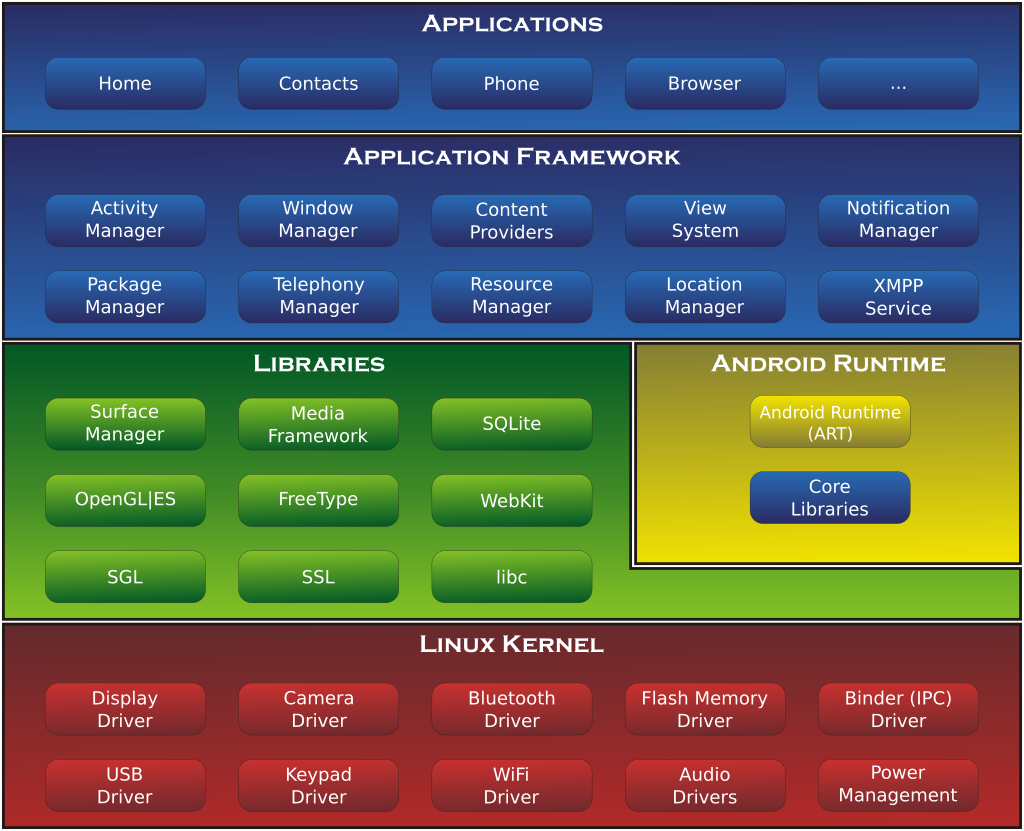
\includegraphics[width=0.7\linewidth]{figs/android_stack.png}
    \caption{Arhitectura sistemului de operare Android}
    \label{fig:android_stack}
\end{figure}

Este cel mai popular sistem de operare pentru dispozitive mobile, fiind fololsit de peste 75 \% din dispozitivele mobile.

\subsection{Capabilitatile de comunicare wireless ale dispozitivelor Android}
Datorita faptului ca Android este gandit in principal pentru dispozitive mobile, acesta ofera o serie de capabilitati de comunicare wireless, precum:
\begin{itemize}
    \item Wi-Fi
    \item Retele mobile
    \item Bluetooth
    \item NFC
\end{itemize}
Documentatia oficiala a Android ofera o serie de API-uri pentru a putea folosi aceste capabilitati in aplicatii: \url{https://developer.android.com/guide/topics/connectivity}
\subsection{Dezvoltarea aplicatiilor Android}
\subsubsection{Android Studio}
Mediul de dezvoltare oficial pentru Android este Android Studio, un IDE bazat pe IntelliJ IDEA, oferind o experienta similara.
Acesta vine cu o serie de facilitati pentru dezvoltarea aplicatiilor Android, precum un emulator pentru dispozitive mobile, un compilator si un depanator.
Poate fi descarcat gratuit de pe site-ul oficial: \url{https://developer.android.com/studio}
\subsubsection{Gradle}
Grade este un build system (asemantor cu Make sau Maven) care vine integrat in Android Studio.
\subsubsection{ADB}
ADB(Andorid Debug Bridge) este un tool care permite comunicarea cu dispozitivele Android, oferind o serie de comenzi pentru a instala aplicatii, a depana sau a face debugging.
\subsubsection{Logcat}
Logcat este un tool care permite vizualizarea log-urilor generate de aplicatii, fiind util pentru depanare.
\section{Creearea unei aplicatii Android}
\subsection{Project template}
Sablonul pentru acest proiect poate fi descarcat de pe GitHub: \url{https://github.com/Dantsz/ProiectTWDM}
\subsubsection{Initializarea proiectului}
\begin{enumerate}
    \item clonati proiectul de pe GitHub
          \begin{lstlisting}
            git clone git@github.com:Dantsz/ProiectTWDM.git
        \end{lstlisting}
    \item deschideti Android Studio
    \item selectati \textit{Open}
    \item selectati directorul in care ati clonat proiectul
          \begin{figure}[H]
              \centering
              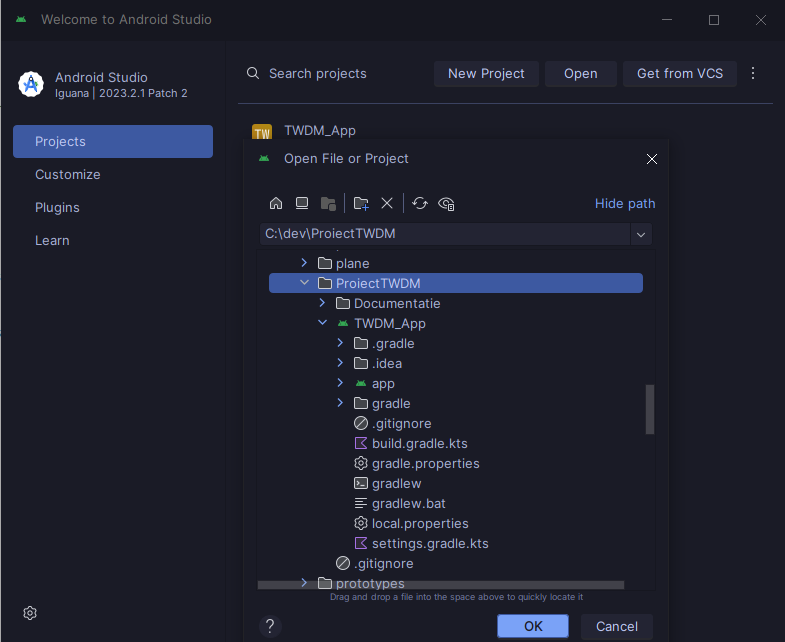
\includegraphics[width=0.7\linewidth]{figs/open_project.png}
              \caption{Deschiderea proiectului}
              \label{fig:open_project}
          \end{figure}
\end{enumerate}
\subsubsection{Structura proiectului}
Un proiect Android are o structura specifica, in care fisierele sunt organizate in directoare specifice.
\begin{itemize}
    \item \texttt{Fisierul manifest} descrie proprietati ale aplicatiei, cum ar fi permisiunile necesare.
    \item \texttt{Folderul kotlin + java} contine codul sursa al aplicatiei.
    \item \texttt{Folderul res} contine fisiere xml care descriu interfata grafica, imagini, string-uri si alte resurse.
\end{itemize}
\paragraph{Model View ViewModel}
Aplicatia foloseste arhitectura MVVM, care separa logica de afisare de logica de business.
\begin{figure}[H]
    \centering
    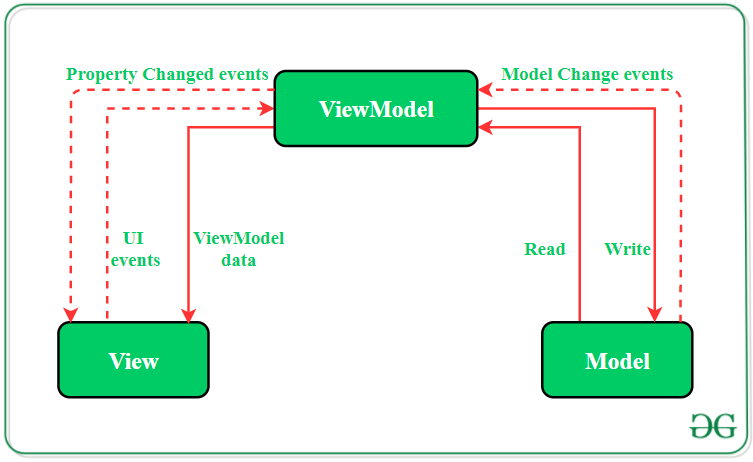
\includegraphics[width=0.7\linewidth]{figs/mvvm.png}
    \caption{Arhitectura MVVM}
    \label{fig:mvvm}
\end{figure}
In contextul acestei aplicatii fiecare fereastra are un ViewModel asociat, care defineste
datele si operatiile care pot fi efectuate pe aceste date.

\subsection{Rulare}
Pentru a rula aplicatia din Android Studio,
controalele implicite sunt: Shift + F10, sau folosind butonul de Run din bara de meniu de sus.
Pentru a selecta dizpovitivul pe care doriti sa rulati aplicatia, puteti folosi butonul de selectie a dispozitivului.
\begin{figure}[H]
    \centering
    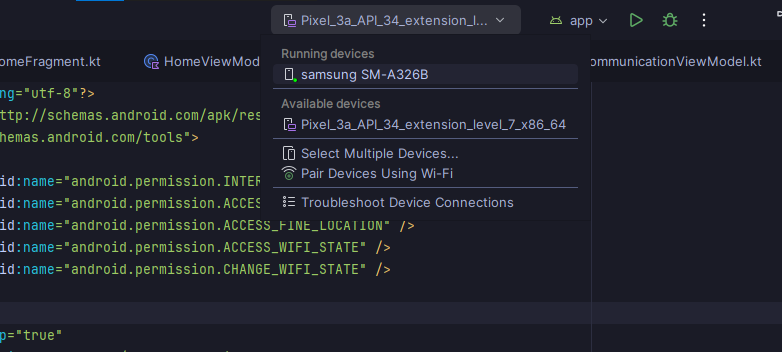
\includegraphics[width=0.7\linewidth]{figs/select_device.png}
    \caption{Selectarea dispozitivului}
    \label{fig:select_device}
\end{figure}
\section{Capacitati de comunicare in rețea utilizand Android}

\subsection{Afisarea informatiilor despre interfetata de retea WiFi}
Pentru a afisa informatii despre interfata de retea WiFi a dispozitivului, trebuie sa folosim clasa \textit{WifiManager}.
Aceasta clasa ne ofera acces la informatii pentru toate aspectele legate de conectivitatea WiFi.
Deoarece aceasta clasa este un serviciu de sistem, trebuie sa obtinem o referinta la aceasta folosind metoda \textit{getSystemService()}.
\begin{lstlisting}[language=Kotlin]
    val wifiManager = this.context?.getSystemService(Context.WIFI_SERVICE) as WifiManager;
\end{lstlisting}
Aceasta clasa contine o proprietate numita \textit{connectionInfo} care ne ofera informatii despre conexiunea WiFi curenta.
\begin{lstlisting}[language=Kotlin]
    val wifiInfo = wifiManager.connectionInfo;
\end{lstlisting}
Daca am apela metoda \textit{toString()} pe acest obiect, am obtine un sir de proprietati separate de virgula.
\begin{lstlisting}[language=Kotlin]
    SSID: "AndroidWifi", BSSID: 00:13:10:85:fe:01, MAC: 02:00:00:00:00:00, IP: /10.0.2.16, Security type: 0, Supplicant state: COMPLETED, Wi-Fi standard: 1, RSSI: -50, Link speed: 1Mbps, Tx Link speed: 1Mbps, Max Supported Tx Link speed: 11Mbps, Rx Link speed: 2Mbps, Max Supported Rx Link speed: 11Mbps, Frequency: 2447MHz, Net ID: 0, Metered hint: false, score: 60, isUsable: true, CarrierMerged: false, SubscriptionId: -1, IsPrimary: -1, Trusted: true, Restricted: false, Ephemeral: false, OEM paid: false, OEM private: false, OSU AP: false, FQDN: <none>, Provider friendly name: <none>, Requesting package name: <none>"AndroidWifi"openMLO Information: , Is TID-To-Link negotiation supported by the AP: false, AP MLD Address: <none>, AP MLO Link Id: <none>, AP MLO Affiliated links: <none>
\end{lstlisting}
Schimband virgulele cu caractere de linie noua, le putem afisa intr-un TextView.
\subsubsection{Afisarea informatiilor in interfata grafica}
\subsubsection{Rezultat}

Ruland programul folosind emulatorul, putem observa informatiile afisate in interfata grafica.

\begin{figure}[H]
    \centering
    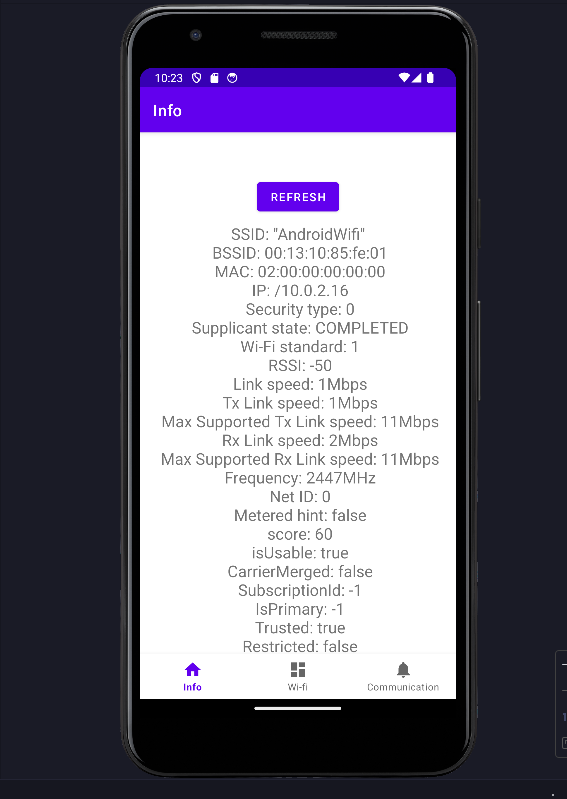
\includegraphics[width=0.7\linewidth]{figs/wifi_info_emulator.png}
    \caption{Informatii despre reteaua WiFi ruland aplicatia in emulator}
    \label{fig:wifi_info}
\end{figure}

Putem observa ca informatiile afisate par a fi "dummy" si nu sunt reale. Acest lucru se datoreaza faptului ca emuleaza o reteta WiFi si un dispozitiv.
Ruland aplicatia pe un telefon fizic putem observa informatii reale despre reteaua WiFi la care este conectat dispozitivul.
\section{Scanarea retelelor Wi-Fi}
\subsection{Scanare}
Pentru a scana punctele de access Wi-Fi la care dispozitivului se poate conecta ne trebuie o referinta la WiFi manager ca si in cazul afisarii informatiilor despre retea.
Vom face scanarea in functia onCreate a fragmetului, adaugand:

\begin{lstlisting}[language=Kotlin]
    val wifiManager = this.context?.getSystemService(Context.WIFI_SERVICE) as WifiManager;
    if (!wifiManager.startScan())
    {
        Log.e("WIFI", "FAILED TO START SCAN OF WIFI APs")
    }
\end{lstlisting}

Pentru a citi rezultatul scanarii trebuie sa folosim un receiver pentru evenimente de
tipul \textit{SCAN\_RESULTS\_AVAILABLE\_ACTION} produse de serviciul de sistem WiFi.

\begin{lstlisting}[language=Kotlin]
    val intentFilter = IntentFilter()
    intentFilter.addAction(WifiManager.SCAN_RESULTS_AVAILABLE_ACTION)
    this.activity?.registerReceiver(wifiScanReceiver, intentFilter)
\end{lstlisting}

Proprietatea wifiScanReceiver este un obiect de tipul \textit{BroadcastReceiver} care va fi definit in fragment.
Trebuie sa suprascriem metoda \texttt{onReceive} pentru a procesa rezultatele scanarii.
Pentru a updata modelul am adaugat si functia \texttt{onScanUpdate} in ViewModel.

\begin{lstlisting}[language=Kotlin]
    private val wifiScanReceiver = object : BroadcastReceiver() {
        override fun onReceive(context: Context, intent: Intent) {
            val success = intent.getBooleanExtra(WifiManager.EXTRA_RESULTS_UPDATED, false)
            if (success) {
                scanSuccess(context)
            } else {
                scanFailure(context)
            }
        }
    }
    @SuppressLint("MissingPermission")
    private fun scanSuccess(context: Context) {
        val wifiManager = context.getSystemService(Context.WIFI_SERVICE) as WifiManager
        val dashboardViewModel =
            ViewModelProvider(this)[DashboardViewModel::class.java]
        val results = wifiManager.scanResults
        dashboardViewModel.onScanUpdate(results)

        Log.i("WIFI", results.toString())
    }

    @SuppressLint("MissingPermission")
    private fun scanFailure(context: Context) {
        val wifiManager = context.getSystemService(Context.WIFI_SERVICE) as WifiManager
        val results = wifiManager.scanResults
        Log.i("WIFI", results.toString())
    }
\end{lstlisting}
\subsection{Afisarea rezultatelor}
Pentru a afisa in interfata grafica rezultatele scanarii trebuie sa folosim un element grafic.
In fragmentul {WifiScan} trebuie sa adaugam un element de tipul \texttt{RecyclerView}:
\begin{lstlisting}[language=XML]
<androidx.constraintlayout.widget.ConstraintLayout xmlns:android="http://schemas.android.com/apk/res/android"
    xmlns:app="http://schemas.android.com/apk/res-auto"
    xmlns:tools="http://schemas.android.com/tools"
    android:layout_width="match_parent"
    android:layout_height="match_parent"
    tools:context=".ui.dashboard.WiFiScanFragment">
    ...
    <androidx.recyclerview.widget.RecyclerView
        android:id="@+id/recyclerView"
        android:layout_width="0dp"
        android:layout_height="0dp"
        android:layout_marginStart="1dp"
        android:layout_marginTop="64dp"
        android:layout_marginEnd="1dp"
        android:layout_marginBottom="50dp"
        app:layout_constraintBottom_toBottomOf="parent"
        app:layout_constraintEnd_toEndOf="parent"
        app:layout_constraintHorizontal_bias="0.0"
        app:layout_constraintStart_toStartOf="parent"
        app:layout_constraintTop_toTopOf="parent"
        app:layout_constraintVertical_bias="0.0" />
</androidx.constraintlayout.widget.ConstraintLayout>
\end{lstlisting}
Pentru a putea transmite datele catre RecyclerView trebuie sa folosim un adaptor si un model pentru un element.
Modelul este o clasa data simpla care contine doar un string:
\begin{lstlisting}[language=Kotlin]
    data class NetworkItemViewModel(val name: String){

    }
\end{lstlisting}
Pentru a folosi RecyclerView trebuie sa definim un element grafic pentru un element din lista.
Acest element grafic este definit intr-un fisier XML separat.
\begin{lstlisting}[language=XML]
<?xml version="1.0" encoding="utf-8"?>
<androidx.cardview.widget.CardView xmlns:android="http://schemas.android.com/apk/res/android"
    android:layout_width="match_parent"
    android:layout_height="50dp"
    android:layout_margin="10dp"
    app:cardElevation="6dp"
    android:layout_marginHorizontal="10dp"
    android:layout_marginVertical="10dp"
    xmlns:app="http://schemas.android.com/apk/res-auto"
    xmlns:tools="http://schemas.android.com/tools"
    >

    <androidx.constraintlayout.widget.ConstraintLayout
        android:layout_width="match_parent"
        android:layout_height="wrap_content">

        <ImageView
            android:layout_width="60dp"
            android:layout_height="60dp"
            android:id="@+id/image"
            android:layout_marginStart="20dp"
            android:padding="8dp"
            android:adjustViewBounds="true"
            android:scaleType="fitXY"
            app:layout_constraintStart_toStartOf="parent"
            app:layout_constraintBottom_toBottomOf="parent"
            app:layout_constraintTop_toTopOf="parent"
            android:src="@drawable/ic_home_black_24dp"
            android:contentDescription="TODO" />
        <TextView
            android:layout_width="wrap_content"
            android:layout_height="wrap_content"
            android:id="@+id/network_name"
            android:textColor="@color/black"
            android:textSize="16sp"
            android:text="Title"
            android:layout_marginStart="20dp"
            app:layout_constraintStart_toEndOf="@id/image"
            app:layout_constraintTop_toTopOf="parent"
            app:layout_constraintBottom_toBottomOf="parent" />
    </androidx.constraintlayout.widget.ConstraintLayout>

</androidx.cardview.widget.CardView>

\end{lstlisting}
Clasa adaptor este o clasa care extinde RecyclerView. Adapter si care primeste ca parametru un ViewHolder.
ViewHolder este o clasa folosita pentru a seta proprietatile elementului grafic cu datele din obiectul de la pozitia corespunzatoare.

\begin{lstlisting}[language=Kotlin]
class NetworkItemAdapter(private val dataList: ArrayList<NetworkItemViewModel>):
    RecyclerView.Adapter<NetworkItemAdapter.ViewHolderClass>() {
    class ViewHolderClass(itemView: View): RecyclerView.ViewHolder(itemView) {
        val nameText: TextView = itemView.findViewById(R.id.network_name)
    }

    override fun onCreateViewHolder(parent: ViewGroup, viewType: Int): ViewHolderClass {
        val view = LayoutInflater.from(parent.context)
            .inflate(R.layout.network_item, parent, false)

        return ViewHolderClass(view)
    }

    override fun getItemCount(): Int {
      return dataList.size
    }

    override fun onBindViewHolder(holder: ViewHolderClass, position: Int) {
        val itemViewModel = dataList[position]
        holder.nameText.text = itemViewModel.name
    }
}
\end{lstlisting}

Acum ca avem dataele si elemetele necesare pentru a afisa rezultatele scanarii, trebuie sa le combinam, vom incepe in clasa de viewmodel, unde vom
adauga lista de retele scanate si o functie care va fi apelata de catre fragment pentru a updata lista.
\begin{lstlisting}
    class WiFiScanViewModel : ViewModel() {

    ...
    private val _scanResults = MutableLiveData<List<ScanResult>>().apply {
        value = ArrayList()
    }
    val scanResults: LiveData<List<ScanResult>> = _scanResults

    fun onScanUpdate(results: MutableList<ScanResult>)
    {
        _scanResults.value = results
    }

\end{lstlisting}

Iar cand view-ul fragmentului este creat, trebuie sa adaugam adaptorul si sa setam datele pentru RecyclerView.
\begin{lstlisting}[language=Kotlin]
    dashboardViewModel.scanResults.observe(viewLifecycleOwner) {
    val data = ArrayList<NetworkItemViewModel>()
    for (i in it)
    {
        data.add(NetworkItemViewModel(i.SSID))
    }
    val adapter = NetworkItemAdapter(data)
    binding.recyclerView.layoutManager = LinearLayoutManager(this.context)
    binding.recyclerView.adapter = adapter
\end{lstlisting}

Acum putem rula aplicatia si putem observa retelele Wi-Fi la care dispozitivul se poate conecta.

\begin{figure}[H]
    \centering
    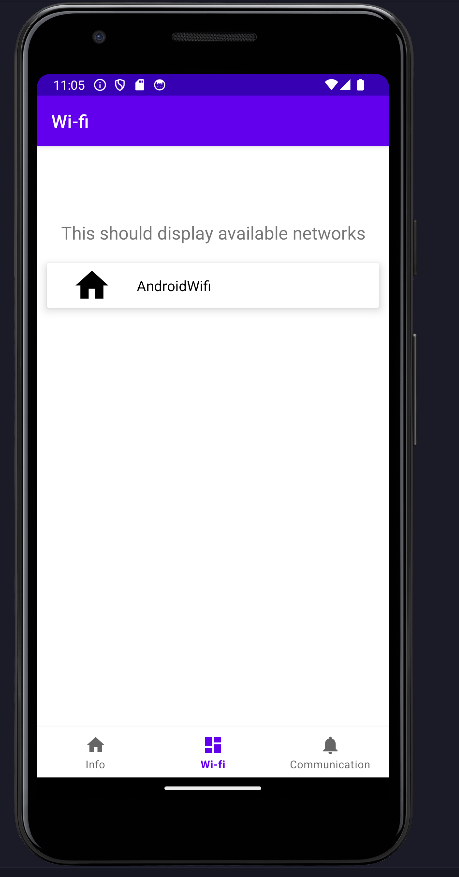
\includegraphics[width=0.7\linewidth]{figs/wifi_scan_res.png}
    \caption{Rezultatele scanarii retelelor Wi-Fi}
    \label{fig:wifi_scan_res}
\end{figure}
\section{Conectarea la un server}
Pentru a evidentia capacitatile de comunicare, vom realiza o conexiune tcp la un server si vom trimite si primi date de la acesta.
\paragraph{Permisiuni} Pentru a realiza conexiuni la internet, trebuie sa adaugam permisiunea in fisierul AndroidManifest.xml:
\begin{lstlisting}[language=XML]
...
<uses-permission android:name="android.permission.INTERNET" />
...
\end{lstlisting}
In fragmentul \texttt{fragment\_communication.xml} am adaugat elementele de interfata necesare pentru a realiza conexiunea la server.
In clasa viewmodel corespunzatoare avem nevoie de un string in care sa stocam raspunsul primit de la server.
Va trebuii sa observam schimbarile din acest string si sa le afisam in interfata grafica.
\begin{lstlisting}[language=Kotlin]
 override fun onCreateView(
        inflater: LayoutInflater,
        container: ViewGroup?,
        savedInstanceState: Bundle?
    ): View {
        ...
        communicationViewModel.response.observe (viewLifecycleOwner) {
            binding.responseText.text = it
        }
        ...
    }
\end{lstlisting}
\paragraph{Conectarea la server} In metoda \texttt{onCreateView} vom adauga un listener pentru butonul de send.
Pentru a realiza conexiunea la server, vom folosi clasa \texttt{Socket}. Deoarece
aceasta clasa nu poate fi folosita in thread-ul principal, vom folosi un thread separat pentru a realiza conexiunea.
\begin{lstlisting}[language=Kotlin]

 binding.button2.setOnClickListener {
            val network_thread = Thread {
                Log.d("WIFI", "Clicked send tcp")
                val address: String = binding.addrText.text.toString()
                val port: Int = binding.portText.text.toString().toInt()
                val connstr = "$address:$port";

                Log.d("WIFI", "Clicked send tcp, connecting to $connstr")
                val client = Socket(address, port)
                Log.d("WIFI", "Sending the message")
                val data = binding.messageText.text.toString() + '\n'
                client.getOutputStream().write(data.toByteArray())
                Log.d("WIFI", "MessageSent, waiting for response")
                val scanner = Scanner(client.getInputStream())
                val resp = scanner.nextLine()
                Log.d("WIFI", "Got response!$resp")
                communicationViewModel.onResponse(resp)
            }
            network_thread.start()
        }
\end{lstlisting}

Valorile pentru adresa si portul serverului sunt citite din interfata grafica, valorile implicite au fost setate pentru conectarea
la serverul \texttt{tcpbin}, care este un server ce returneaza datele primite, acestea trebuie sa fie terminate cu un caracter de newline.

\begin{figure}[H]
    \begin{subfigure}{0.5\textwidth}
        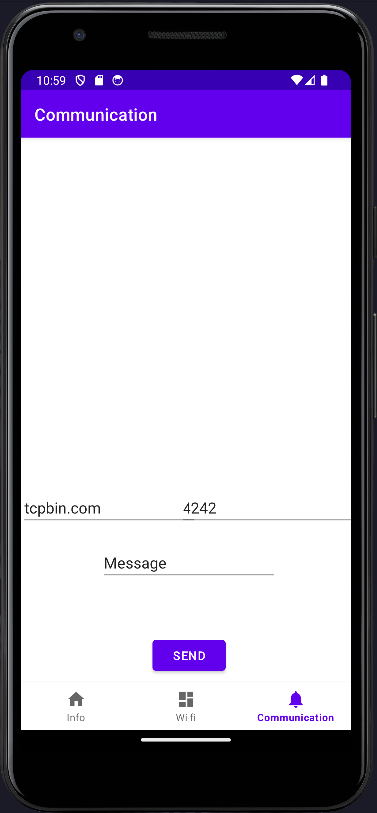
\includegraphics[width=\textwidth]{figs/comm_before.png}
    \end{subfigure}
    \hfill
    \begin{subfigure}{0.5\textwidth}
        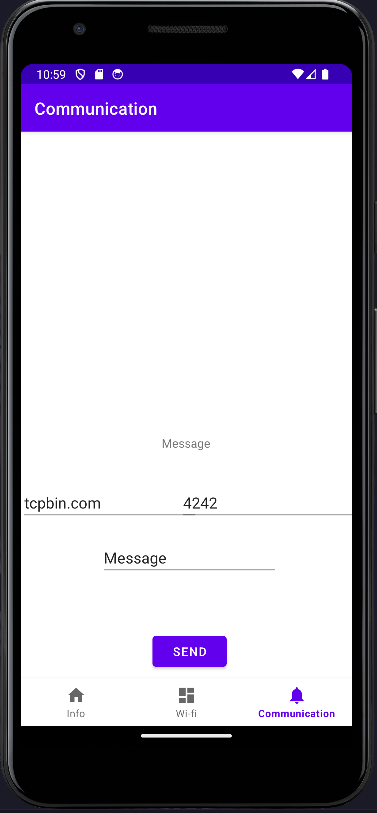
\includegraphics[width=\textwidth]{figs/comm_after.png}
    \end{subfigure}
\end{figure}
%\bibliography{twdm}
\end{document}